% !TEX encoding = UTF-8
% !TEX TS-program = pdflatex
% !TEX root = ../tesi.tex

%**************************************************************
\chapter{Introduzione}
\label{cap:introduzione}
%**************************************************************

\section{Sommario}\label{sec: Sommario}

Il presente documento descrive il lavoro che ho svolto durante il periodo di stage, della durata di 304 ore, presso l'azienda G-Squared Srl di Ponte San Nicolò (PD).
\\
Il progetto di stage prevedeva l'analisi, la progettazione e lo sviluppo di un \emph{widget} Qt (elemento principale per la creazione di interfacce utente in Qt) che permetta la visualizzazione 3D volumetrica di una ricostruzione fatta tramite immagini diagnostiche medicali radiologiche, catturate tramite TC (Tomografia computerizzata) o RM (Risonanza magnetica).
\\
Questo elaborato ha lo scopo di illustrare il contesto aziendale dove è stato svolto lo stage, le attività svolte durante esso, ed infine una valutazione sul lavoro effettuato.

\begin{figure}[ht]
    \centering
    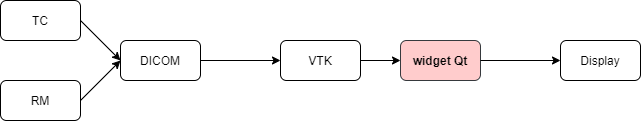
\includegraphics[width=1\textwidth]{immagini/schemainiziale.png}
    \caption{\textit{Sequenza dei componenti: in evidenza l'oggetto principale del lavoro}}
    \label{fig: Intro Scheme}
\end{figure}

Nella figura \ref{fig: Intro Scheme} possiamo vedere la sequenza dei componenti: dall'esame radiologico svolto tramite TC o RM che genera i file DICOM, al loro caricamento nella libreria VTK. Il risultato viene quindi elaborato e mostrato nel \emph{widget} Qt, aspetto principale del lavoro di stage, per essere mostrato a schermo.

%**************************************************************
\section{Organizzazione del testo}

Il testo è così suddiviso:
\begin{itemize}
    \item \hyperref[cap:introduzione]{Il primo capitolo} introduce il contenuto della tesi e descrive l'organizzazione del testo;
    \item \hyperref[cap:descrizione-stage]{Il secondo capitolo} descrive l'azienda, gli obiettivi dello stage, le tecnologie e gli strumenti utilizzati;
    \item \hyperref[cap:teoria-stage]{Il terzo capitolo} descrive la teoria e gli algoritmi alla base del \emph{volume rendering}, con menzione alle librerie utilizzate;
    \item \hyperref[cap:resoconto-stage]{Il quarto capitolo} descrive l'esperienza effettuata nella progettazione e nello sviluppo del progetto di stage;
	\item \hyperref[cap:conclusioni]{Il quinto capitolo} presenta una valutazione dello stage in relazione agli obiettivi dell'azienda e all'esperienza da me acquisita nel corso del suo svolgimento.
\end{itemize}


Riguardo la stesura del testo, relativamente al documento sono state adottate le seguenti convenzioni tipografiche:
\begin{itemize}
	\item gli acronimi, le abbreviazioni e i termini ambigui o di uso non comune menzionati vengono definiti nel loro primo utilizzo;
	\item i termini in lingua straniera o facenti parti del gergo tecnico sono evidenziati con il carattere \emph{corsivo}.
\end{itemize}